
\documentclass{article}

% required packages
\usepackage[usenames,dvipsnames]{color}
\usepackage[nottoc,notlot,notlof]{tocbibind}
\usepackage[toc]{glossaries}
\usepackage{amsmath}
\usepackage{listings} 
\usepackage{graphicx}
\usepackage{wrapfig}

\definecolor{grey}{rgb}{0.9,0.9,0.9}
\lstset{%
basicstyle=\footnotesize,
backgroundcolor=\color{grey},}

\title{\textcolor{red}{COMMODORE 64 TITLE}}
\author{CSC 350 - Project 1 \\ Daniel Savage - V00701453}
\date{January/February 2014}

\begin{document}
   \maketitle
   
\pagebreak{}

\tableofcontents

\pagebreak{}
   
\section{Introduction}
foo foo bar

\section{The architecture}

\subsection{Overview}

\subsection{Memory}

\subsubsection{RAM}

\subsubsection{Color RAM}

\subsubsection{ROM}

\subsubsection{Memory Map}

\subsection{MOS 6510 CPU}
\paragraph{}
The Commodore 64's microprocessor is the MOS Technology 6510, a variant of the 6502 model. Leading up to the years of the Commodore 64's production, the MOS 6502 had become substantially popular in home computer architecture for its comprehensive features while having a fraction of the price of its competitors. This section will describe the Commodore 64's 6510 in two sections. The first being its general features that is has in common with with the 6502, and the second being its unique characteristics.

\subsubsection{6502 Family Features}

\paragraph{}
The MOS Technology 6502 is a little-endian 8-bit microprocessor with a 16-bit address bus. The 6502 was designed with a two-phase clock design, implementing a very primitive form of pipelining. While an address can be accessed during the first clock phase of the 6502, data can be retrieved during the second from a previous access, allowing two instructions to happen somewhat asynchronously. 

\paragraph{}
The 6502's design can be considered quite minimalistic compared to other designs of its time, such as the Intel 8080. Taking advantage of the fact that memory speeds were much faster CPU clocks at the time of production, the architecture focuses on storing data outside of the processor. Most programming techniques focus on having an accumulator register that is manipulated with various elements from memory. The 6502 has only seven registers: the accumulator (A), two index registers (X, Y), a status register (P), stack pointer (SP), and a double-width, 16-bit program counter (PC). The address space of the stack exists over $\mathtt{\$0100 - \$01FF}$, giving 256 bytes for programming. 

\paragraph{}
The 6502 assembly language is often considered \textit{fun} compared to other varieties of instructions, such as x86. This can often be attributed to the fact that it was inherently designed to be programmed by hand, and less so by an automated compiler. Instructions more or less focus on exchanging or modifying the accumulator with some location in memory, making very straightforward code. A table of common opcodes can be seen here:
    \begin{center}
    \begin{tabular}{|p{2cm}|p{5cm}|p{2cm}|p{5cm}|}
    \hline
    OPCODE & FUNCTION                                       & OPCODE & FUNCTION                                                   \\ \hline
    LDA \#00       & put an immediate value into the accumulator    & ADC \$0110     & add a value from memory into the accumulator with carry    \\ \hline
    LDA \$0110     & load a value from memory into the accumulator  & SBC \$0111     & subtract a value from memory from the accumulator          \\ \hline
    STA \$0111     & store a value from memory into the accumulator & AND \$10       & logical AND function with either memory or immediate value \\ \hline
    LDX \#00       & put an immediate value into the X register     & CMP \$0112     & compare memory and the accumulator                         \\ \hline
    \end{tabular}
    \end{center}

\paragraph{}
An example program is listed below, which doubles a number in the accumulator until it is greater than a specified number in the X register.

\begin{lstlisting}
LDA #01 ; put an unsigned value of 1 into the accumulator
STA $0200 ; store the value in memory
LDX #100 ; put an unsigned limit of 100 into the X register
double: 
LDA $0200 ; load from memory
ADC $0200 ; add the value to itself
STA $0200 ; store the new sum back into memory
CPX $0200 ; compare the value with X
BCC double ; double again until the value is no longer less than X
\end{lstlisting}

\paragraph{}
The 6502 family of microprocessors also has a form of fast zero page addressing modes. Addresses $\mathtt{\$00FF - \$00FF}$ only required a single byte to query memory, allowing for faster access. Zero page addressing could be applied by the assembly programmer by specifying address size as follows.
\begin{lstlisting}
LDA $0F ; load memory $000F using zero page addressing (faster)
LDA $000F ; load memory $000F using normal addressing (slower)
\end{lstlisting}

\pagebreak

\subsubsection{6510 Specific Features}
\paragraph{}
\begin{wrapfigure}{l}{0.35\textwidth}
\vspace{-20pt}
\caption{6510 pin layout}
\begin{center}
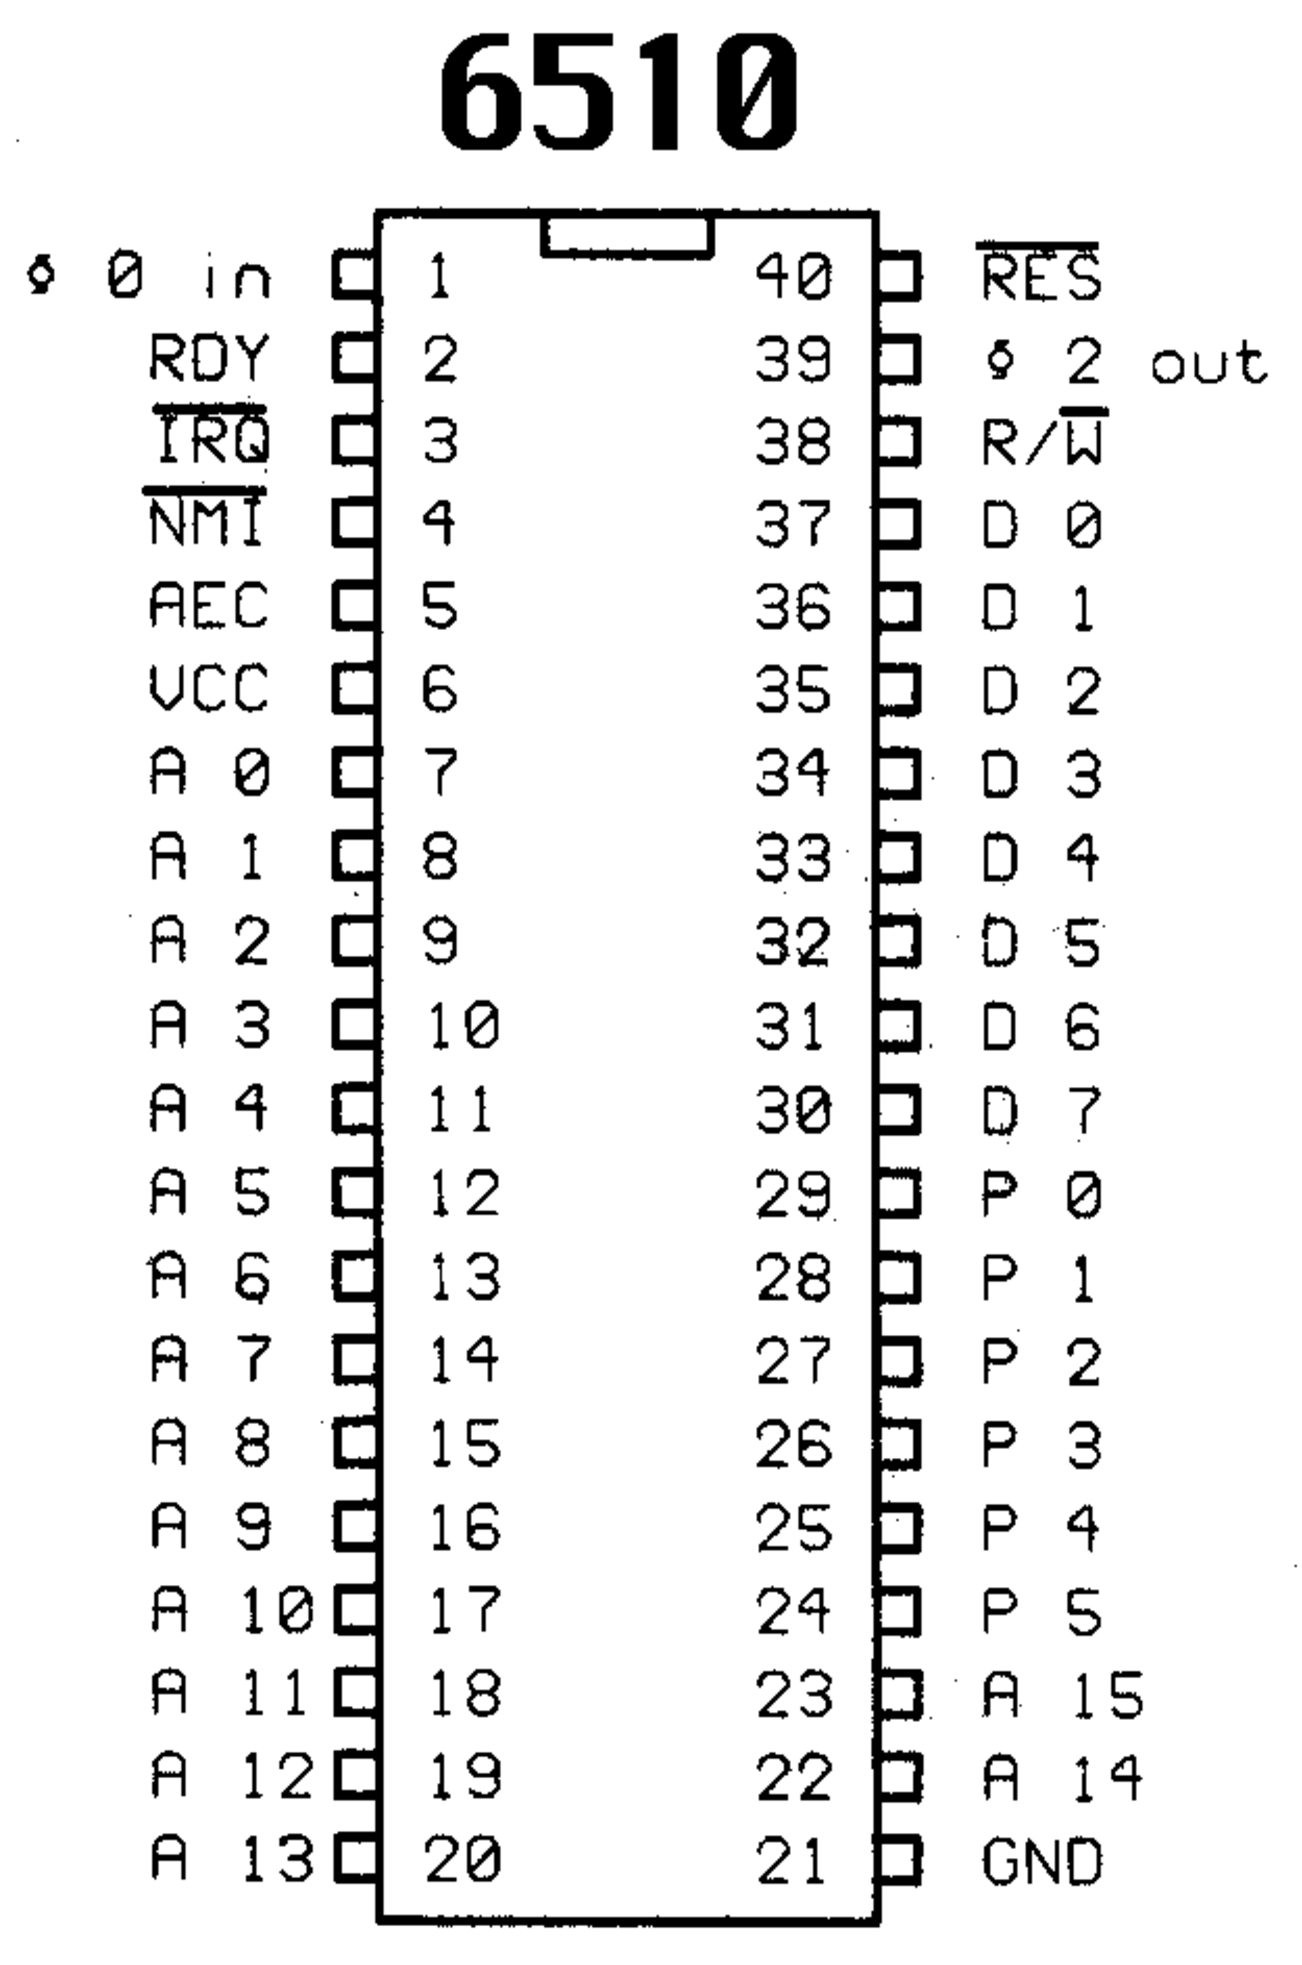
\includegraphics[width=3cm]{6510}
\end{center}
\end{wrapfigure}
The MOS Technology 6510 is a variant of the 6502 microprocessor, accompanied with an I/O port of either six or eight bits wide. The Commodore 64 uses the 6-bit version of this port to interact switch between RAM and ROM, as well as access to tertiary memory, such as a datacasette. The 6510 can also make its address lines become tristate, allowing it to share memory with other devices, such as the SID and the VIC-II. Since RAM, ROM, and I/O registers are all mapped to the same address space, the Commodore 64 can distinguish between the three through the $P0$ and $P1$ lines for accessing ROM, and the $P2$ line for the I/O registers. $P3$, $P4$, and $P5$ are used to operate the datacasette.


\subsection{MOS 6567 VIC-II}
asdasd

\subsection{MOS 6581 SID}
adasdasdasd

\subsection{MOS 6526 CIA}
asdasdas

\section{Strengths}

\section{Weaknesses}

\section{Critical analysis}

\section{Conclusion}

\pagebreak

\begin{thebibliography}{9}

\bibitem{lamport94}
  Leslie Lamport,
  \emph{\LaTeX: A Document Preparation System}.
  Addison Wesley, Massachusetts,
  2nd Edition,
  1994.

\end{thebibliography}

\end{document}